\documentclass[12pt, a4paper]{article}
\usepackage[utf8]{inputenc}
\usepackage{graphicx, hyperref, float, adjustbox, amsmath, subcaption}




% Update this information to reflect yourself
\title{Assignment 1: Three- \& Four-Sum Problem}
\author{Christian Vilen}
\date{2022-09-20}

\begin{document}
\maketitle

\section{Introduction}
The Three-Sum and Four-Sum problem is a classic computer science challenge in the area of algorithm design and implementation. The objective of the Three-Sum challenge is to determine if three distinctive elements exist within a data structure that sum up to zero when added together. This is extended to one more distinctive element in the Four-Sum Challenge. The Three-Sum problem satisfies the following mathematical properties:
\[i, j, k \, (i \neq j, \, i \neq k, \, j \neq k), \, \, x_i + x_j + x_k = 0\]

This academic paper aims to report on three different implementations that solve the Three-Sum and Four-Sum problem. Accordingly, the comparison should highlight their respective performance complexity characteristics with various tables and figures.

\section{Implementation}

The implementation of the solutions to the Three-Sum and Four-Sum problems can be found in the code repository here: \href{https://github.com/C-Vilen/ITU_Applied_Algo_2023/tree/main/ThreeFourSum}{Git Repository}.
The time and space complexity can be seen for all implementations in the below table:
\begin{table}[H]
  \begin{center}
    \begin{adjustbox}{max width=0.7\textwidth}
      \begin{tabular}{|c|c|c|c|}
        \begin{tabular}{rrrr}
    Algorithm & Implementation & Time Complexity & Space Complexity \\\hline
    Three-Sum & Cubic & $O(n^3)$ & $O(1)$\\
             & Quadratic & $O(n^2)$ & $O(1)$\\
             & HashMap & $O(n^2)$ & $O(n)$\\\\\hline
    Four-Sum & Quartic & $O(n^4)$ & $O(1)$\\
     & Cubic & $O(n^3)$ & $O(1)$\\
     & HashMap & $O(n^2)$ & $O(n^2)$\\
\end{tabular}
    
      \end{tabular}
    \end{adjustbox}
    \caption{The time and space complexity denoted for each algorithm.}
    \label{tbl:threeFourSumComplexityTable}
  \end{center}
\end{table}


\subsection{Hardware and Software Specification}
All of the experiments have been executed on the following equipment:
\begin{itemize}
\item Computer: MacBook Pro, 14-inch 2021, Apple M1 Pro, 16 GB RAM.
\item OS: Mac OS X Ventura 14.0
\item Software: Java: 17.0.5 2022-10-18 LTS, JUnit: 4.13.2, Python: 3.11.5, Gradle: 7.6 \& Kotlin: 1.7.10
\end{itemize}
The computer performing the tests has been connected to a wall power outlet during the benchmarking of the algorithms to ensure maximum power output from the CPU.

\subsection{Correctness Tests}
The implementation of the four different Three-Sum and Four-Sum algorithms has been tested with various JUnit tests to verify their correctness. This includes multiple variable test cases of 0, 1 and more triplets summing to null or not.
\newline
It is also important to note, that the tests for the ThreeSumHashMapMissingComparison() method are to show the importance of the \texttt{\&\& j < k} condition in the HashMap implementation as it ensures \(x_i, x_j\) and \(x_k\) are at distinctive positions in the input array.

\subsection{Input Data}
The data generated for the tests of the different solutions of the Three-Sum and Four-Sum problem has used the following mathematical expression:
\[n_i = 30 \cdot 1.41^i\;\text{, } i \text{ was set to 30.}\]
This is in order to produce an approximate increasing factor of \(\sqrt{2}\) for every element in the input data. Hereby, providing a sufficient incremental scale and range of data.
\newline
Please note the minimum heap size for Java has been increased to 8 GB in the Python experiments script in order to accommodate the OutOfMemoryError exception. This error occurred around the \(30 \cdot 1.41^{25}\) which typically gave an OutOfMemoryError exception on the larger input data on the HashMap implementation for the Four-Sum problem and random OutOfMemoryError exception side-effects on some arbitrary input data.


\section{Experiments}
\subsection{Three-Sum Experiments}
The three solutions to the Three-Sum problem have an increasing average execution time as the input size increases. This is the expected behaviour for each of the respective solutions which can be seen in Figure~\ref{threesumTableFigure}. The Cubic solution has the slowest execution time compared to the two other solutions in Figure~\ref{fig:threeruntimes} which also matches the time complexity in  table~\ref{tbl:threeFourSumComplexityTable} in chapter 2 "Implementation" of \(O(n^3)\). This can also be deducted from the table~\ref{tbl:three_average} as it increases drastically once it reaches the interval of 931 to 7321 elements where after it hits the 30-second time limit. The HashMap solution performs an intermediate between the two other solutions as seen in Figure~\ref{fig:threeruntimes}. Notably, even though it has a running time of \(O(n^2)\) like the Quadratic solution, it also has to create the actual HashMap data structure which takes \(O(n)\) space complexity. Therefore, the Quadratic solution performs the best compared to the other solutions as it only takes space complexity of \(O(1)\) enabling it to handle a bigger input of values. This can also be analysed in the table~\ref{tbl:three_average}.
\begin{figure}[H]
  \begin{subfigure}{0.59\textwidth} 
    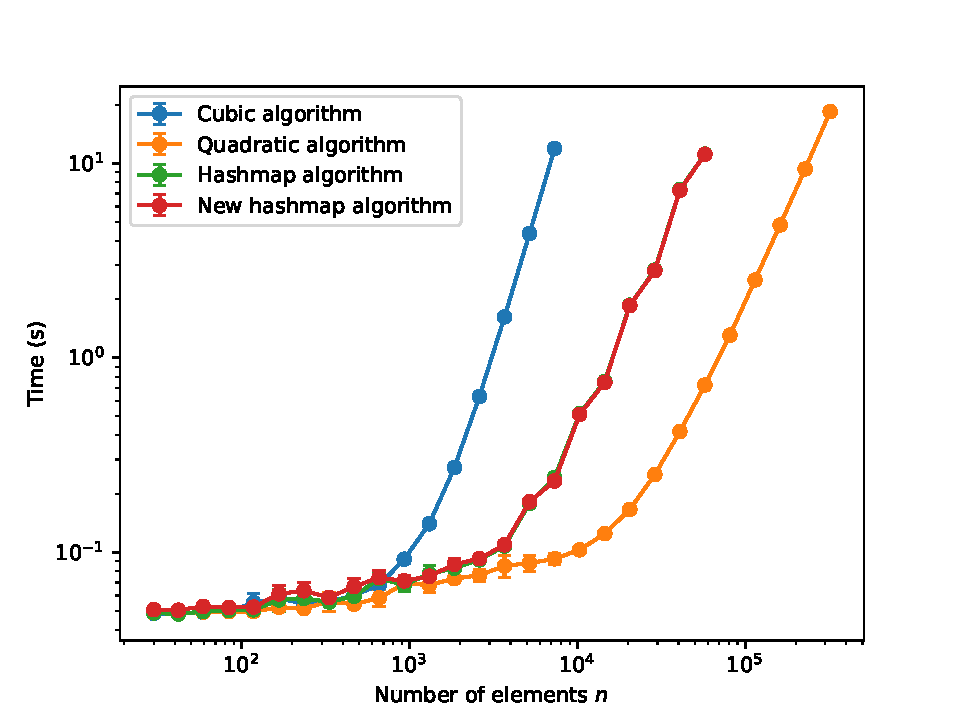
\includegraphics[width=\textwidth]{three_sum.pdf}
    \subcaption{Three-Sum running time visualized}
    \label{fig:threeruntimes}
  \end{subfigure}
  \hfill
  \begin{subfigure}{0.40\textwidth}
    \begin{adjustbox}{max width=\textwidth}
      \begin{tabular}{|c|c|c|c|}
        \begin{tabular}{rrrr}
    &	Quadratic	&	HashMap	&	Cubic	\\\hline
    $n$	&	Average (s)	&	Average (s)	&	Average (s)	\\\hline
    30	&	0.063505	&	0.059988	&	0.061507	\\
    42	&	0.061963	&	0.059843	&	0.059706	\\
    59	&	0.062234	&	0.060554	&	0.059845	\\
    84	&	0.059868	&	0.060749	&	0.060798	\\
    118	&	0.059056	&	0.061999	&	0.070067	\\
    167	&	0.059508	&	0.0696	&	0.072669	\\
    235	&	0.060454	&	0.066129	&	0.067609	\\
    332	&	0.061804	&	0.066078	&	0.066479	\\
    468	&	0.067846	&	0.077522	&	0.069739	\\
    660	&	0.077953	&	0.079692	&	0.07929	\\
    931	&	0.079583	&	0.075003	&	0.098821	\\
    1313	&	0.084588	&	0.078429	&	0.15172	\\
    1852	&	0.082476	&	0.083722	&	0.284409	\\
    2611	&	0.084126	&	0.101965	&	0.658235	\\
    3682	&	0.080772	&	0.118165	&	1.724355	\\
    5192	&	0.082349	&	0.195614	&	4.496418	\\
    7321	&	0.091411	&	0.25034	&	12.346113	\\
    10323	&	0.105925	&	0.527608	&	-	\\
    14556	&	0.140508	&	0.777544	&	-	\\
    20525	&	0.18033	&	1.902266	&	-	\\
    28940	&	0.269289	&	2.878875	&	-	\\
    40805	&	0.417973	&	7.414434	&	-	\\
    57536	&	0.729295	&	11.447228	&	-	\\
    81126	&	1.377281	&	-	&	-	\\
    114387	&	2.546927	&	-	&	-	\\
    161286	&	4.983893	&	-	&	-	\\
    227414	&	9.691578	&	-	&	-	\\
    320654	&	18.88899	&	-	&	-	\\
\end{tabular}
      \end{tabular}
    \end{adjustbox}
    \subcaption{Average running time for\\each Three-Sum implementa-\\tion.}
    \label{tbl:three_average}
  \end{subfigure}
  \caption{Figure and table for Three-Sum implementations}
  \label{threesumTableFigure}
\end{figure}

\subsection{Four-Sum Experiments}
The Four-Sum problem increases the time complexity across all of the solutions as it adds one more element to the challenge. This can be seen in the smaller amount of elements which has been tested against each solution in figure~\ref{foursumTableFigure}. The Quartic solution performs the worst as it uses a time complexity of \(O(n^4)\) as also highlighted in table~\ref{tbl:threeFourSumComplexityTable} in chapter 2 "Implementation". The average running time table~\ref{tbl:four_average} also highlights the larger running time for the Quartic solution as it only reaches 1313 elements before it encounters the 30-second time limit. Interestingly, the HashMap and Cubic solutions perform rather similarly when looking at the figure~\ref{fig:fourruntimes} even though they have different time complexity of \(O(n^2)\) and \(O(n^3)\), respectively. The HashMap solution manages to perform a benchmark with the largest input of elements for the Four-Sum problem of 10323 elements. However, as mentioned in Chapter 2.3 "Input Data" the minimum heap size for Java was increased to handle the larger input data because it threw an OutOfMemoryError exception. This is due to the space complexity that the HashMap solution utilises of \(O(n^2)\) to create the actual HashMap data structure. Thus, presents the important argument that time complexity cannot solely be the determinator to analyse any algorithm as the space complexity also has to be considered. \newline The Cubic solution performs rather similarly to the HashMap solution on the smaller data input as seen in table~\ref{tbl:four_average} until it reaches 5192 elements where the impact of its time complexity of \(O(n^3)\) takes effect. Accordingly, the Cubic solution would arguably become slower intensively if the time limit was increased hereby diverging further from the HashMap solution.

\begin{figure}[H]
  \begin{subfigure}{0.58\textwidth} 
    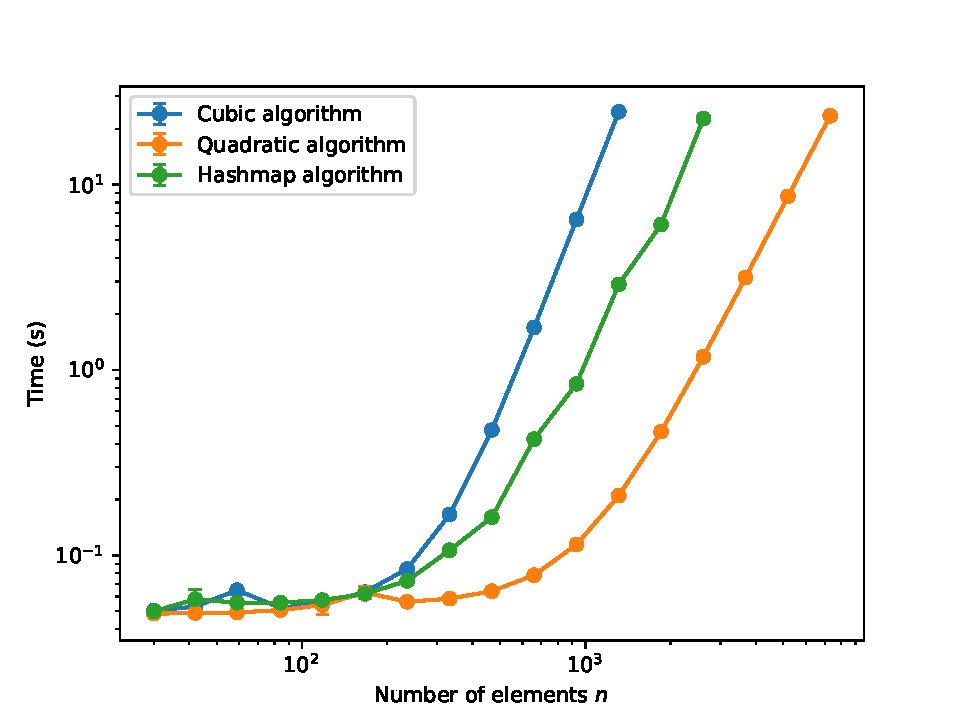
\includegraphics[width=\textwidth]{four_sum.pdf}
    \subcaption{Four-Sum running time visualised}
    \label{fig:fourruntimes}
  \end{subfigure}
  \hfill
  \begin{subfigure}{0.40\textwidth}
    \begin{adjustbox}{max width=\textwidth}
      \begin{tabular}{|c|c|c|c|}
        \begin{tabular}{rrrr}
    &	HashMap	&	Cubic	&	Quartic	\\\hline
    $n$	&	Average (s)	&	Average (s)	&	Average (s)	\\\hline
    30	&	0.06003	&	0.059621	&	0.062323	\\
    42	&	0.060648	&	0.060944	&	0.065905	\\
    59	&	0.061434	&	0.061416	&	0.07585	\\
    84	&	0.067853	&	0.062963	&	0.068966	\\
    118	&	0.075652	&	0.070409	&	0.065506	\\
    167	&	0.079377	&	0.077767	&	0.07342	\\
    235	&	0.104045	&	0.06685	&	0.094405	\\
    332	&	0.094721	&	0.069491	&	0.178064	\\
    468	&	0.101786	&	0.074724	&	0.497435	\\
    660	&	0.106156	&	0.090133	&	1.752576	\\
    931	&	0.141698	&	0.12693	&	6.648049	\\
    1313	&	0.238788	&	0.222236	&	25.285927	\\
    1852	&	0.561357	&	0.484803	&	-	\\
    2611	&	1.623853	&	1.204709	&	-	\\
    3682	&	3.511084	&	3.209423	&	-	\\
    5192	&	5.92609	&	8.863057	&	-	\\
    7321	&	12.712385	&	24.261229	&	-	\\
    10323	&	27.181545	&	-	&	-	\\
\end{tabular}
      \end{tabular}
    \end{adjustbox}
    \subcaption{Average running time for\\each Four-Sum implementation.}
    \label{tbl:four_average}
  \end{subfigure}
  \caption{Figure and table for Four-Sum implementations}
  \label{foursumTableFigure}
\end{figure}

\end{document}